\documentclass[landscape,paperwidth=46truein,paperheight=41truein,fontscale=0.3]{baposter}
\usepackage{graphics}
\usepackage{color}
\usepackage{multicol}
\usepackage{amsmath}
\usepackage{amssymb, wasysym}
\usepackage{epstopdf}
\usepackage{graphicx}
\usepackage{tikz}
\usepackage[small,labelfont=bf,up,textfont=it,up]{caption}
\usepackage{contour}
\usepackage{enumitem}
\usepackage{array}
\usepackage{calc}
\usepackage{siunitx}

\newenvironment{nscenter}
{\parskip=0pt\par\nopagebreak\centering}
{\par\noindent\ignorespacesafterend}

\begin{document}
\definecolor{myfavoritecolor}{rgb}{2.55 0.25 0.0}
\small
\contourlength{1pt} %how thick each copy is
\contournumber{20}  %number of copies
\lefthyphenmin4
\righthyphenmin4
%\fontdimen2\font=0.2ex% inter word space

%:Background image
\background{
	\begin{tikzpicture}[remember picture,overlay]%
	\draw (current page.center)+(-0em,-13.5em) node[anchor=center]
	{\includegraphics[width=1.2\textwidth]{Images/aia171_blue}};
	\end{tikzpicture}%
}

\begin{poster}
{%Keyword=value pairs
  % Color style
  bgColorOne=black,
  bgColorTwo=black,
  background = user,
  borderColor=darkgray,
  headerColorOne=black,
  headerColorTwo=gray,
  headerFontColor=white,
  boxColorOne=white,
  boxColorTwo=myfavoritecolor,
  % Format of textbox
  textborder=roundedleft,
  % Format of text header
  eyecatcher=true,
  headerborder=closed,
  headerheight=0.18\textheight,
  headershape=roundedright,
  headershade=shadelr,
  boxshade=plain,
  headerfont=\LARGE\textrm,
}
{%Eyecatcher
   \resizebox{!}{.13\textheight}{
\includegraphics{Images/NASA_logo.png}}
}
{%Poster Title
   \contour{black}{\color{white} Measuring Doppler Shifts in the Transition Region}
}
{%Author
		\contour{black}{\color{white}Roy Smart, Charles C.\ Kankelborg} \\
		\contour{black}{\color{white}Physics Department, Montana State University, Bozeman, MT 59717}\\
		\contour{black}{\color{white}roy.smart@montana.edu } \\
}
{%Logo
   \resizebox{!}{.18\textheight}{
\includegraphics{Images/inverted_solar_physics_logo}}
}

%%%%%%%%%%%%%%%%%%%%%%%%%%%%%%%%%%%%
%         Zeroth Column            %
%%%%%%%%%%%%%%%%%%%%%%%%%%%%%%%%%%%%

\headerbox{Abstract}{name=abstract,column=0}{
\vspace{0.02 \columnwidth}
\begin{center}
	\begin{minipage}{0.95\columnwidth}
		The measurement of Doppler shift in solar emission lines %in the solar atmosphere 
		%is an important plasma diagnostic which 
		is essential for the determination of the bulk flow velocity of the solar atmosphere. Measuring this quantity over a 2D field-of-view with high spatial, spectral and temporal resolution is important for 
		%initializing and verifying 
		driving and testing
		models of the solar atmosphere, but 
		%has proven to be a difficult observational problem. 
		current instruments are incapable of achieving this in EUV and FUV.
		Using a computed tomography imaging spectrograph known as MOSES 
		(Multi-Order Solar EUV Spectrograph)
		and an inversion algorithm utilizing convolutional neural networks, we develop a technique to recover the Doppler shift over a wide field-of-view with arcsecond resolution. We apply this technique to the data from the MOSES I flight.
	\end{minipage}
\end{center}
\vspace{0.00 \columnwidth}
}

\headerbox{\textit{MOSES} Instrument}{name=MOSES Instrument, column=0,below=abstract, above=bottom}{
\vspace{5pt}
\begin{center}
	\begin{minipage}{0.95\columnwidth}

		The slit employed by traditional spectrographs 
		%is important as it 
		allows the spectrum of any given slice of the sun to be interpreted unambiguously. However, 
		%observing the Sun through a narrow slit can be prohibitive, as 
		because of the slit,
		two-dimensional views of the Sun can only be acquired through the process of rastering
		, which
		confuses space and time. 
		While rastering is adequate for 2D characterization of events with timescales much longer than the exposure time of the instrument, events on smaller timescales must be observed using a different method.
		
%		Removing the slit employed by a traditional spectrograph allows us to trade spectral bandwidth for spatial
		
		\hspace{8pt} MOSES is an instrument that recovers spectral information over a wide 2D field-of-view by removing the slit employed by traditional spectrographs. This design choice overlaps spatial and spectral information onto an imaging sensor.
		%, trading spectral bandwidth for spatial bandwidth by using a narrow passband. 
		Deprojection of space and spectrum along the MOSES dispersion direction is a problem in computed tomography, which we make easier by choosing a narrow passband dominated by a single spectral line, He\,\textsc{ii} $\lambda 304$\,\AA.
		Computational inversion algorithms are applied to images at three diffraction orders to separate the spatial/spectral information and recover spectral information over a large 2D area of the Sun.
		
%		\hspace{8pt} The dense object of Figure \ref{invert} can always be inverted using the three orders. Unfortunately, general extended objects cannot be uniquely determined and must use physical constraints to deproject space and spectra.
		
		\begin{center}		
			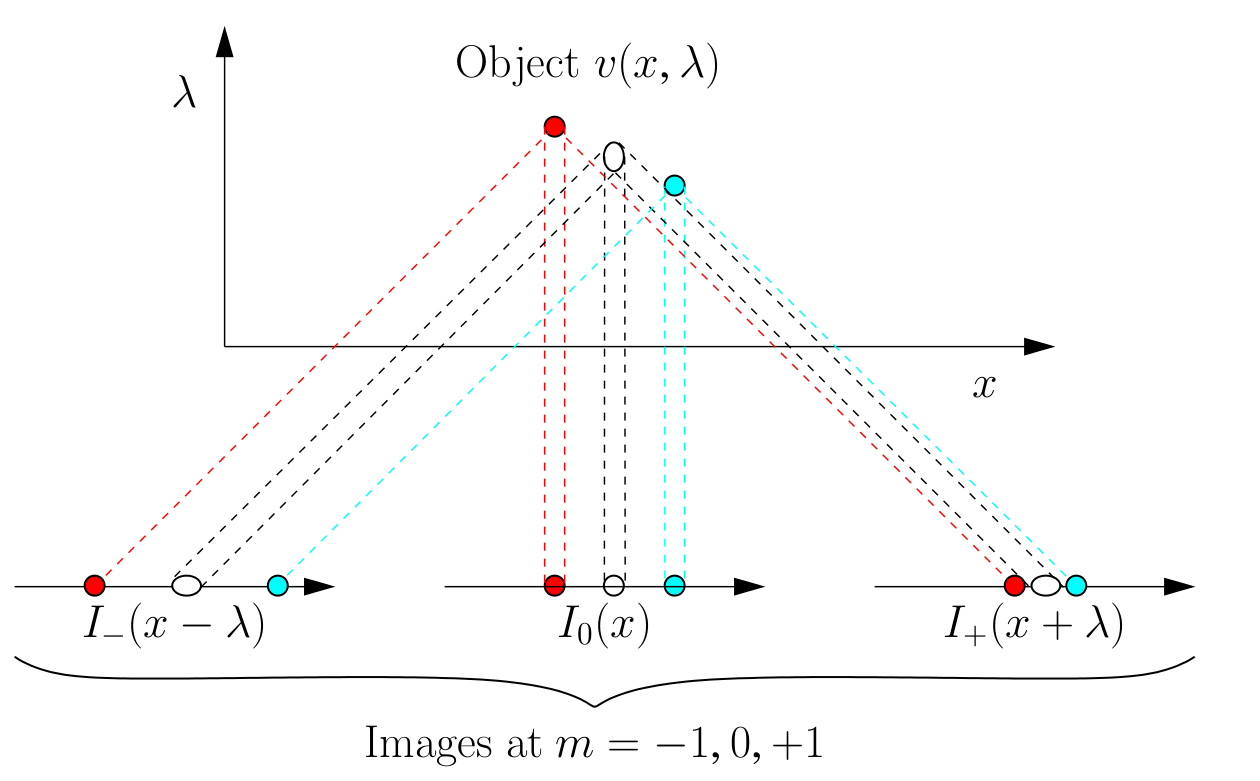
\includegraphics[width=0.9\columnwidth]{Images/inversion}
			\captionof{figure}{\label{invert}Visualization describing how MOSES projects spectral and spatial information onto a imaging sensor [1]. A dense object in $x-\lambda$ space appears to have relative shifts as imaged from different diffraction orders. This operation is generally non-invertible, and physical constraints must be used to limit the possible interpretations of MOSES images} 		  
		\end{center} 

	\end{minipage}
\end{center}
}   



%%%%%%%%%%%%%%%%%%%%%%%%%%%%%%%%%%%%
%          First Column            %
%%%%%%%%%%%%%%%%%%%%%%%%%%%%%%%%%%%%

\headerbox{Doppler Shift Inversion Neural Network}{name=doppler, column=1,span=3}{

	\begin{center}
		\begin{minipage}{0.98 \columnwidth}
			
			\begin{multicols}{3}
				In principle, information could be extracted from MOSES observations by using a forward model of MOSES and previous spectral observations to construct a dictionary of spectral features and their corresponding MOSES signature. Observations could then be matched to entries in this dictionary to recover spectral information.
				
				%A brute-force approach to extracting information from MOSES observations is to use a forward model of MOSES and previous spectral observations to construct a dictionary of spectral features and their corresponding MOSES signature. Observations could then be matched to entries in this dictionary to recover spectral information.
				
				\hspace{8pt} We can approximate the above brute-force approach using a convolutional neural network. Tradtional neural networks can approximate an arbitrary vector-valued function, $\mathbf{f(\mathbf{x})}$, by using weighted combinations of nonlinear, monotonic functions of the input $\mathbf{x}$. %Our neural network is convolutional, meaning that it is shift-invariant.
				 %basis elements. 
				 The weights form a set of free parameters and are found through an optimization procedure known as training, where the network is presented with enough example points on $\mathbf{f}(\mathbf{x})$ as required for convergence. Neural networks are often layered to increase the number of free parameters and thus the quality of the approximation. If $\mathbf{f}(\mathbf{x})$ is translation invariant (as for the MOSES inversion), it is appropriate to use convolutional neural networks where a number of small neural networks (called filters) are convolved with the input vector to approximate $\mathbf{f}(\mathbf{x})$ while maintaining the property of translation invariance.
				
				\hspace{8pt} We implemented a convolutional neural network to estimate the Doppler shift as a function of two MOSES images. %Since they are both low transition region lines, 
				  %Si \textsc{iv} \SI{1403}{\angstrom} line 
				  Spectra from the \textit{Interface Region Imaging Spectrograph} (IRIS) were taken as an analogue to the MOSES He\,\textsc{ii} line to train the network. Si\,\textsc{iv} was chosen because of the abundantly available spectra for training. While Si\,\textsc{iv} is formed differently from He\,\textsc{ii}, both exhibit complex line profiles typical of lower transition region dynamics. The first moment in the spectral dimension of the IRIS observations was defined as the true Doppler shift and was used to direct training.
				
				\hspace{8pt} In Figure \ref{conv_vis} we can see the operation of a simple version of our network.  Each row contains a flattened 3D filter (weight matrix) and a 2D slice of an `activation cube' (AC). Each slice of the AC is found by performing a 3D convolution on the AC below. The colors associate slices of the 3D kernel with the appropriate slice of the AC.
			

			\begin{center}
			\setlength{\tabcolsep}{.1em} % for the horizontal padding
			{\renewcommand{\arraystretch}{0.5}% for the vertical padding
			\begin{tabular}{| p{1in} | r |} \hline
				 Original Image
				 &
				\begin{tabular}{c c c c | c}
					& & & & 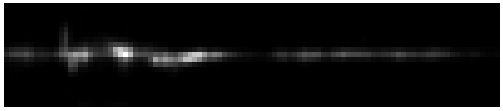
\includegraphics[width=1in]{../../../../src/python/minnd/model_plt/img_0_2_0_0}
				\end{tabular} \\ \hline
				 
 				 Forward Model
 				 &
			 	\begin{tabular}{c c c c | c}
					& & & & 
\includegraphics[width=1in]{../../../../src/python/minnd/model_plt/img_1_2_0_0}\\
					& & & &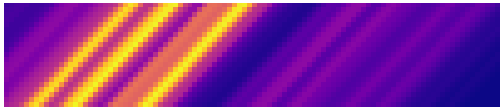
\includegraphics[width=1in]{../../../../src/python/minnd/model_plt/img_1_2_1_0}
 				 \end{tabular} \\ \hline
				 				 
				 Layer 1
				 &
				\begin{tabular}{c c c c | c}
					
\includegraphics[height=0.2in]{../../../../src/python/minnd/model_plt/img_w} &
					
\includegraphics[height=0.2in]{../../../../src/python/minnd/model_plt/img_w} &
					
\includegraphics[height=0.2in]{../../../../src/python/minnd/model_plt/img_2_1_0_0} &
					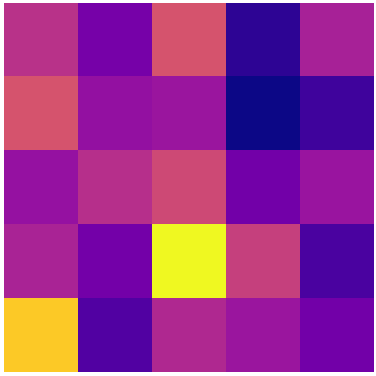
\includegraphics[height=0.2in]{../../../../src/python/minnd/model_plt/img_2_1_0_1} & 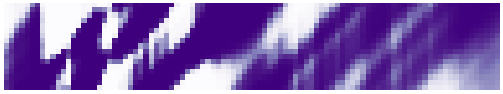
\includegraphics[width=1in]{../../../../src/python/minnd/model_plt/img_2_2_0_0} \\ \hline
					
\includegraphics[height=0.2in]{../../../../src/python/minnd/model_plt/img_w} &
					
\includegraphics[height=0.2in]{../../../../src/python/minnd/model_plt/img_w} &
					
\includegraphics[height=0.2in]{../../../../src/python/minnd/model_plt/img_2_1_1_0} &
					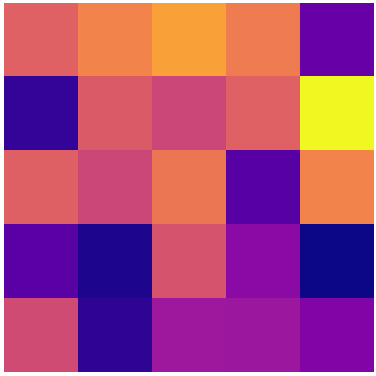
\includegraphics[height=0.2in]{../../../../src/python/minnd/model_plt/img_2_1_1_1} & 
\includegraphics[width=1in]{../../../../src/python/minnd/model_plt/img_2_2_1_0} \\ \hline
					
\includegraphics[height=0.2in]{../../../../src/python/minnd/model_plt/img_w} &
					
\includegraphics[height=0.2in]{../../../../src/python/minnd/model_plt/img_w} &
					
\includegraphics[height=0.2in]{../../../../src/python/minnd/model_plt/img_2_1_2_0} &
					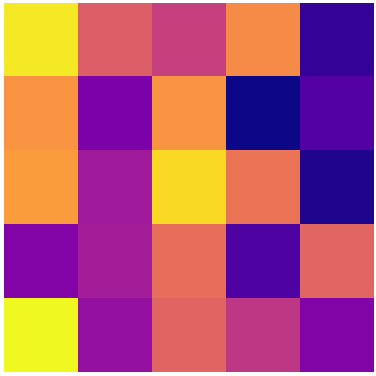
\includegraphics[height=0.2in]{../../../../src/python/minnd/model_plt/img_2_1_2_1} & 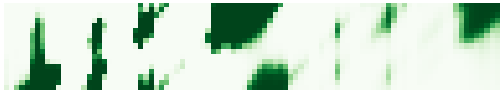
\includegraphics[width=1in]{../../../../src/python/minnd/model_plt/img_2_2_2_0} \\
				 \end{tabular} \\ \hline
				 				 				 
				 Layer 2
				 &
				\begin{tabular}{c c c c | c}
					
\includegraphics[height=0.2in]{../../../../src/python/minnd/model_plt/img_w} &
					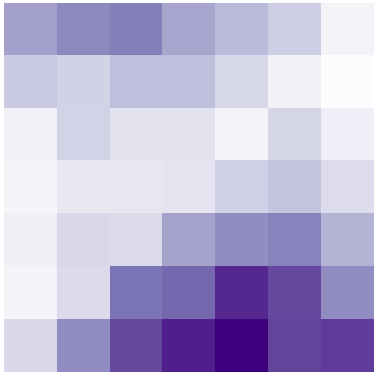
\includegraphics[height=0.2in]{../../../../src/python/minnd/model_plt/img_3_1_0_0} &
					
\includegraphics[height=0.2in]{../../../../src/python/minnd/model_plt/img_3_1_0_1} &
					
\includegraphics[height=0.2in]{../../../../src/python/minnd/model_plt/img_3_1_0_2} & 
\includegraphics[width=1in]{../../../../src/python/minnd/model_plt/img_3_2_0_0} \\ \hline
					
\includegraphics[height=0.2in]{../../../../src/python/minnd/model_plt/img_w} &
					
\includegraphics[height=0.2in]{../../../../src/python/minnd/model_plt/img_3_1_1_0} &
					
\includegraphics[height=0.2in]{../../../../src/python/minnd/model_plt/img_3_1_1_1} &
					
\includegraphics[height=0.2in]{../../../../src/python/minnd/model_plt/img_3_1_1_2} & 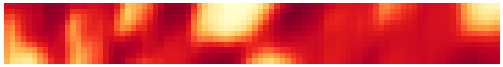
\includegraphics[width=1in]{../../../../src/python/minnd/model_plt/img_3_2_1_0} \\ \hline
					
\includegraphics[height=0.2in]{../../../../src/python/minnd/model_plt/img_w} &
					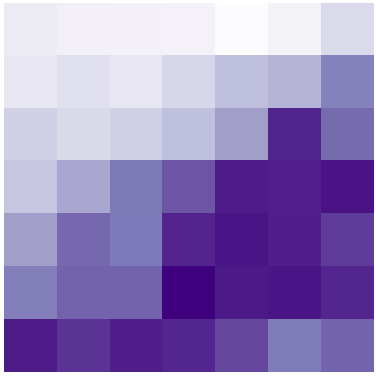
\includegraphics[height=0.2in]{../../../../src/python/minnd/model_plt/img_3_1_2_0} &
					
\includegraphics[height=0.2in]{../../../../src/python/minnd/model_plt/img_3_1_2_1} &
					
\includegraphics[height=0.2in]{../../../../src/python/minnd/model_plt/img_3_1_2_2} & 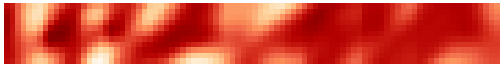
\includegraphics[width=1in]{../../../../src/python/minnd/model_plt/img_3_2_2_0} \\ \hline
					
\includegraphics[height=0.2in]{../../../../src/python/minnd/model_plt/img_w} &
					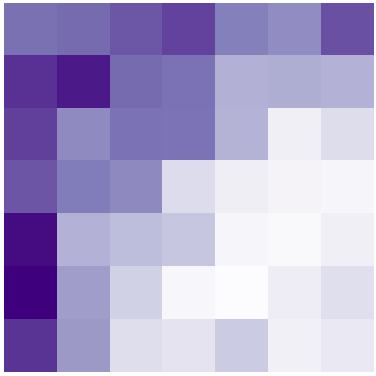
\includegraphics[height=0.2in]{../../../../src/python/minnd/model_plt/img_3_1_3_0} &
					
\includegraphics[height=0.2in]{../../../../src/python/minnd/model_plt/img_3_1_3_1} &
					
\includegraphics[height=0.2in]{../../../../src/python/minnd/model_plt/img_3_1_3_2} & 
\includegraphics[width=1in]{../../../../src/python/minnd/model_plt/img_3_2_3_0} \\
				 \end{tabular} \\ \hline
				 
				 Layer 3
				 &
			 	\begin{tabular}{c c c c | c}
			 		
\includegraphics[height=0.2in]{../../../../src/python/minnd/model_plt/img_4_1_0_0} &
			 		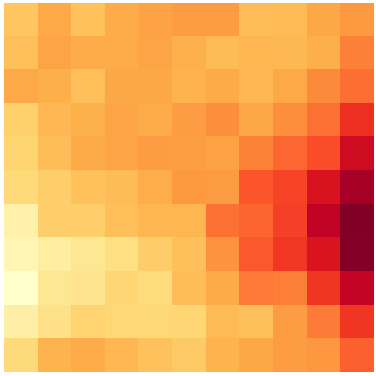
\includegraphics[height=0.2in]{../../../../src/python/minnd/model_plt/img_4_1_0_1} &
			 		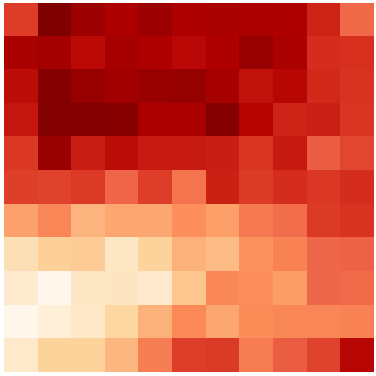
\includegraphics[height=0.2in]{../../../../src/python/minnd/model_plt/img_4_1_0_2} &
			 		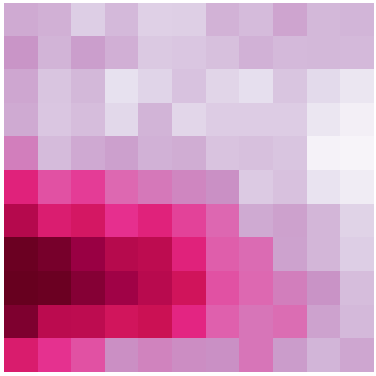
\includegraphics[height=0.2in]{../../../../src/python/minnd/model_plt/img_4_1_0_3} & 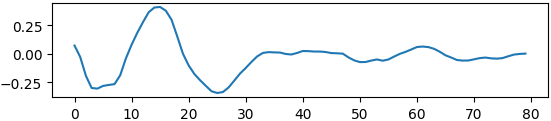
\includegraphics[width=1in]{../../../../src/python/minnd/model_plt/img_4_2_0_0} \\ 
				 \end{tabular} \\ \hline
				

				
			\end{tabular}
			}
			\captionof{figure}{\label{conv_vis}Demonstration of a simple Doppler inversion convolutional neural network.}
			\end{center}
			
		\end{multicols}
		\end{minipage}	
	\end{center}
	\vspace{2pt}
}

\headerbox{Validation}{name=valid, column=1,span=2, below=doppler}{
	\vspace{2pt}
	\begin{center}
		\begin{minipage}{0.975 \columnwidth}
			\begin{multicols}{3}
%				\begin{center}
					{\setlength{\tabcolsep}{.05em} % for the horizontal padding
					\renewcommand{\arraystretch}{0.2}% for the vertical padding
					\begin{tabular}{c}
						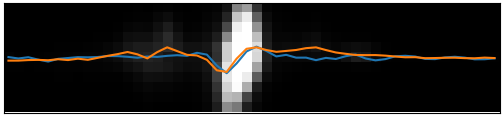
\includegraphics[width=\linewidth]{../../../../src/python/minnd/validation/doppler_1182} \\
						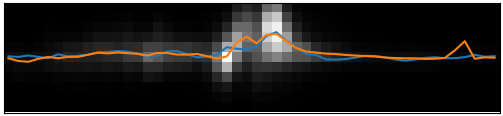
\includegraphics[width=\linewidth]{../../../../src/python/minnd/validation/doppler_1225} \\
						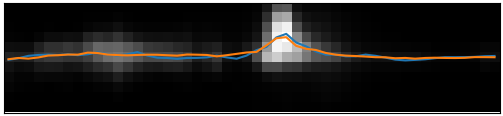
\includegraphics[width=\linewidth]{../../../../src/python/minnd/validation/doppler_1263} \\
						\includegraphics[width=\linewidth]{../../../../src/python/minnd/validation/doppler_1298} \\
						\includegraphics[width=\linewidth]{../../../../src/python/minnd/validation/doppler_1343} \\ 
%						\includegraphics[width=\linewidth]{../../../../src/python/minnd/validation/doppler_1407} \\
%						\includegraphics[width=\linewidth]{../../../../src/python/minnd/validation/doppler_1436} \\
%						\includegraphics[width=\linewidth]{../../../../src/python/minnd/validation/doppler_1797} \\
					\end{tabular}}
%				\end{center}
				
%				\begin{center}
					\centering
					\begin{tabular}{|l c c|} 
						\hline
						& Test & Final \\ \hline
						free parameters & 1.2k & 836k \\
						training images & 4.5k & 4.5k \\ 
						RMS error (km/s) & 12.7 & 10.3\\
						correlation & 0.500 & 0.701\\ \hline	
					\end{tabular}	
					\captionof{table}{(Above) Comparing the performance of the test network used in Figure \ref{conv_vis} and the final network used in the rest of this presentation.} 	
%				\end{center}	
				\captionof{figure}{(Left) The value of the true Doppler velocity (orange) is plotted against the recovered Doppler velocity (blue) over the original IRIS image, rebinned into MOSES pixels} 
				
				\includegraphics[width=0.965\linewidth]{../../../../src/python/minnd/validation/linearity}
				\captionof{figure}{(Above) Histogram plotting the true velocity against the recovered velocity for the 25\% most intense synthetic MOSES pixels in the validation dataset.} 
				
					
					

					
				
			\end{multicols}
		\end{minipage}
	\end{center}
	\vspace{-5pt}
}

\headerbox{Results}{name=results, column=1,span=2, below=valid, above=bottom}{
	\vspace{2pt}
	\begin{center}
		\begin{minipage}{0.97 \columnwidth}
			\begin{multicols}{2}
%				\includegraphics[width=\linewidth]{../../../../src/python/minnd/movies/full/intensity/zero/fig_14} \\
	%					\includegraphics[width=\linewidth]{../../../../src/python/minnd/movies/full/velocity/zero-ave/fig_14} \\
	
				\resizebox{\columnwidth}{!}{%
					\includegraphics[height=10cm]{../../../../src/python/minnd/movies/full/intensity-velocity/zero-ave/fig_14}
					\includegraphics[height=10cm]{../../../../src/python/minnd/movies/full/intensity-velocity/zero-ave/legend} 
				}				
				
				\captionof{figure}{Dopplergram of frame 21 of the 2005 MOSES I observation generated by taking the average result of our method applied to the zero-plus and the zero-minus image combinations.  The vertical scale on the legend indicates velocity in units of km/s and the horizontal scale indicates intensity in arbitrary units. Spatial units are in arcsec\label{full}. Solar north is directed upward.}
				
				{
				\setlength{\tabcolsep}{.05em} % for the horizontal padding
				\renewcommand{\arraystretch}{0.5}% for the vertical padding
				\begin{tabular}{c c c c c c }
					
%					
					
					
					Fox &
					\includegraphics[width=0.185\linewidth]{../../../../src/python/minnd/movies/fox/intensity/minus/fig_14} &
					\includegraphics[width=0.185\linewidth]{../../../../src/python/minnd/movies/fox/intensity/zero/fig_14} &
					\includegraphics[width=0.185\linewidth]{../../../../src/python/minnd/movies/fox/intensity/plus/fig_14} &
					\includegraphics[width=0.185\linewidth]{../../../../src/python/minnd/movies/fox/velocity/zero-ave/fig_14} &
					\includegraphics[width=0.185\linewidth]{../../../../src/python/minnd/movies/fox/intensity-velocity/zero-ave/fig_14} \\
					
					1 &
					\includegraphics[width=0.185\linewidth]{../../../../src/python/minnd/movies/ar1/intensity/minus/fig_00} &
					\includegraphics[width=0.185\linewidth]{../../../../src/python/minnd/movies/ar1/intensity/zero/fig_00} &
					\includegraphics[width=0.185\linewidth]{../../../../src/python/minnd/movies/ar1/intensity/plus/fig_00} &
					\includegraphics[width=0.185\linewidth]{../../../../src/python/minnd/movies/ar1/velocity/zero-ave/fig_00} &
					\includegraphics[width=0.185\linewidth]{../../../../src/python/minnd/movies/ar1/intensity-velocity/zero-ave/fig_00} \\
					
					2 &
					\includegraphics[width=0.185\linewidth]{../../../../src/python/minnd/movies/ar2/intensity/minus/fig_00} &
					\includegraphics[width=0.185\linewidth]{../../../../src/python/minnd/movies/ar2/intensity/zero/fig_00} &
					\includegraphics[width=0.185\linewidth]{../../../../src/python/minnd/movies/ar2/intensity/plus/fig_00} &
					\includegraphics[width=0.185\linewidth]{../../../../src/python/minnd/movies/ar2/velocity/zero-ave/fig_00} &
					\includegraphics[width=0.185\linewidth]{../../../../src/python/minnd/movies/ar2/intensity-velocity/zero-ave/fig_00} \\
					
%					3 &
%					\includegraphics[width=0.185\linewidth]{../../../../src/python/minnd/movies/ar3/intensity/minus/fig_00} &
%					\includegraphics[width=0.185\linewidth]{../../../../src/python/minnd/movies/ar3/intensity/zero/fig_00} &
%					\includegraphics[width=0.185\linewidth]{../../../../src/python/minnd/movies/ar3/intensity/plus/fig_00} &
%					\includegraphics[width=0.185\linewidth]{../../../../src/python/minnd/movies/ar3/velocity/zero-ave/fig_00} &
%					\includegraphics[width=0.185\linewidth]{../../../../src/python/minnd/movies/ar3/intensity-velocity/zero-ave/fig_00} \\
%					
%					4 &
%					\includegraphics[width=0.185\linewidth]{../../../../src/python/minnd/movies/ar4/intensity/minus/fig_00} &
%					\includegraphics[width=0.185\linewidth]{../../../../src/python/minnd/movies/ar4/intensity/zero/fig_00} &
%					\includegraphics[width=0.185\linewidth]{../../../../src/python/minnd/movies/ar4/intensity/plus/fig_00} &
%					\includegraphics[width=0.185\linewidth]{../../../../src/python/minnd/movies/ar4/velocity/zero-ave/fig_00} &
%					\includegraphics[width=0.185\linewidth]{../../../../src/python/minnd/movies/ar4/intensity-velocity/zero-ave/fig_00} \\
					
					& $I_{-1}$ & $I_{0}$ & $I_{1}$ & $v_d$ & $(I_0, \; v_d)$ \\
%					& $I_{0}$ & $v_d$ & $(I_0, \; v_d)$ \\
					
				\end{tabular}
				\vspace{2pt}
				\captionof{figure}{Magnified regions of frame 21 of the MOSES I dataset. From left to right: the $m=-1,0,+1$ MOSES images, Doppler velocity map, intensity-velocity map.} 
			}
				
				
			\end{multicols}

				
%			
		\end{minipage}
	\end{center}
}




%%%%%%%%%%%%%%%%%%%%%%%%%%%%%%%%%%%%
%          Third Column            %
%%%%%%%%%%%%%%%%%%%%%%%%%%%%%%%%%%%%

\headerbox{Discussion}{name=conclusion,column=3, below=doppler}{
	\vspace{5pt}
	\begin{center}
		\begin{minipage}{0.95 \columnwidth}
		
			The results appear to be reasonably smooth in both time and space. There are a myriad of dynamic events to watch over the 15 frames of the observation. Possibly the most interesting is that this method highlights loops, which may provide a robust technique for tracking and isolating loops. 

			\hspace{8pt}The main source of error in this result is the non-trivial MOSES point-spread-function (PSF). The PSF introduces astigmatism into the outboard orders that can be erroneously interpreted as a Doppler shift. For this analysis, no attempt was made to mitigate the effects of the PSF, so these results are only valid on scales larger than the PSF (about 9 MOSES pixels). Mitigating this source of error is an important goal for future work.
			
			\hspace{8pt}The Doppler shifts yielded by our analysis are all much slower than the sound speed. This is in contrast to earlier results from [1] and [2] that recover velocities comparable to the sound speed, especially for impulsive events such as the Fox event.
			
			\hspace{8pt} In future work we aim to find higher moments of transition region spectra using MOSES and its successor the \textit{EUV Snapshot Imaging Spectrograph} (ESIS), expected to fly in 2018.

		\end{minipage}
	\end{center}
	\vspace{0pt}
}


\headerbox{References}{name=refs,column=3,below=conclusion}{
\vspace{2pt}
\footnotesize
\begin{minipage}{\columnwidth}
	\begin{enumerate}[topsep=0pt,itemsep=-1ex,partopsep=1ex,parsep=1ex,leftmargin=*,label={[\arabic*]}]
			\item Fox, J.\ L., Kankelborg, C.\ C., \& Thomas, R.\ J.\ (2010) \textit{APJ}  719, 1132.		 
			\item Courrier, H.\ T., \&  Kankelborg, C.\ C.\ (Oct. 15, 2015) \textit{Proc. SPIE 9643} doi:10.1117/12.2194607			
	\end{enumerate}
\end{minipage}
}

\headerbox{Acknowledgment}{name=ack,column=3,below=refs, above=bottom}{ 
	\footnotesize
	\vspace{2pt}
	\begin{center}
		\begin{minipage}{0.95\columnwidth}
			This work is supported by NASA grant NNX07AG76G\\
		\end{minipage}
	\end{center}
	\footnotesize
}

\end{poster}
\end{document}